\documentclass[aspectratio=169]{beamer}
\usetheme{Bruno}
\usepackage{amsmath}
\usepackage{amssymb}
\usepackage{siunitx}
\usepackage{float}
\usepackage{tikz}
\def\checkmark{\tikz\fill[scale=0.4](0,.35) -- (.25,0) -- (1,.7) -- (.25,.15) -- cycle;} 
\usepackage{url}
\usepackage[siunitx,american,RPvoltages]{circuitikz}
\ctikzset{capacitors/scale=0.7}
\ctikzset{diodes/scale=0.7}
\usepackage{tabularx}
\newcolumntype{C}{>{\centering\arraybackslash}X}
\renewcommand\tabularxcolumn[1]{m{#1}}% for vertical centering text in X column
\usepackage{tabu}
\usepackage[spanish,es-tabla,activeacute]{babel}
\usepackage{babelbib}
\usepackage{booktabs}
\usepackage{pgfplots}
\usepackage{hyperref}
\hypersetup{colorlinks = true,
            linkcolor = black,
            urlcolor  = blue,
            citecolor = blue,
            anchorcolor = blue}
\usepgfplotslibrary{units, fillbetween} 
\pgfplotsset{compat=1.16}
\usepackage{bm}
\usetikzlibrary{arrows, arrows.meta, shapes, 3d, perspective, positioning,mindmap,trees,backgrounds}
\renewcommand{\sin}{\sen} %change from sin to sen
\usepackage{bohr}
\setbohr{distribution-method = quantum,insert-missing = true}
\usepackage{elements}
\usepackage{verbatim}
\usepackage[edges]{forest}
\usepackage{etoolbox}
\usepackage{schemata}
\usepackage{appendix}
\usepackage{listings}

\definecolor{color_mate}{RGB}{255,255,128}
\definecolor{color_plas}{RGB}{255,128,255}
\definecolor{color_text}{RGB}{128,255,255}
\definecolor{color_petr}{RGB}{255,192,192}
\definecolor{color_made}{RGB}{192,255,192}
\definecolor{color_meta}{RGB}{192,192,255}
\newcommand\diagram[2]{\schema{\schemabox{#1}}{\schemabox{#2}}}

\definecolor{codegreen}{rgb}{0,0.6,0}
\definecolor{codegray}{rgb}{0.5,0.5,0.5}
\definecolor{codepurple}{rgb}{0.58,0,0.82}
\definecolor{backcolour}{rgb}{0.95,0.95,0.92}

\lstdefinestyle{mystyle}{
    backgroundcolor=\color{backcolour},   
    commentstyle=\color{codegreen},
    keywordstyle=\color{magenta},
    numberstyle=\tiny\color{codegray},
    stringstyle=\color{codepurple},
    basicstyle=\ttfamily\footnotesize,
    breakatwhitespace=false,         
    breaklines=true,                 
    captionpos=b,                    
    keepspaces=true,                 
    numbers=left,                    
    numbersep=5pt,                  
    showspaces=false,                
    showstringspaces=false,
    showtabs=false,                  
    tabsize=2
}

\lstset{style=mystyle}
\title{Instrumentación I: \\ \emph{Mediciones de}\\ \emph{Temperatura}}
\author{
    Juan J. Rojas, Hugo Sanchez Ortiz
}
\institute{Instituto Tecnológico de Costa Rica}
\date{\today}
\background{fig/background.jpg}
% Change vertical spacing
\renewcommand{\arraystretch}{1.25}
\begin{document}
\sisetup{unit-math-rm=\mathrm,math-rm=\mathrm} % change sinitx font
\sisetup{output-decimal-marker = {,}}
\maketitle
\newcommand{\blackandwhite}{white} %change this at the end

\begin{frame}{Definición de Temperatura}
    \begin{columns}[c, onlytextwidth]
        \begin{column}{0.50\textwidth}
            \begin{itemize}
                \item La temperatura es una manifestación del promedio de energía cinética, ondulatoria y de traslación de las moléculas de una sustancia.
                \item Es una propiedad física que determina si un sistema se encuentra o no en equilibrio térmico con otros sistemas (Ley cero de la termodinámica)
            \end{itemize}
        \end{column}
        \begin{column}{0.45\textwidth}
        \begin{tikzpicture}[
roundnode/.style={circle, draw=black, fill=white, very thick, minimum size=20mm},
squarednode/.style={rectangle, draw=red!60, fill=red!5, very thick, minimum size=15mm},
sqnode/.style={rectangle, draw=blue!60, fill=blue!5, very thick, minimum size=15mm},
snode/.style={rectangle, draw=white, fill=white, very thick, minimum size=15mm},
]
%Nodes
\node[roundnode]      (maintopic)                              {};
\node[squarednode] (leftsquare)       [left=of maintopic] {T\textsubscript{h}};
\node[sqnode]      (rightsquare)       [right=of maintopic] {T\textsubscript{c}};
\node[right=0.5,above] at (leftsquare.east){\small Q\textsubscript{h}};
\node[right=-0.5,above] at (rightsquare.west){\small Q\textsubscript{c}};
\node[snode]      (downsquare)       [below=of maintopic] {\textbf{W}};

%Lines

\draw[->] (maintopic.east) -- (rightsquare.west);
\draw[->] (leftsquare.east) -- (maintopic.west);
\draw[->] (leftsquare.east) -- (maintopic.west);
\draw[->] (maintopic.south)-- (downsquare.north);

\end{tikzpicture}
\newline
\newline
            \tiny{Ciclo de la máquina térmica descrita por Carnot, , el calor entra al sistema a través de una temperatura inicial (aquí se muestra como T\textsubscript{h}) y fluye a través del mismo obligando al sistema a ejercer un trabajo sobre sus alrededores, y luego pasa al medio frío, el cual tiene una temperatura final (T\textsubscript{c}).}
        \end{column}
    \end{columns}
\end{frame}
\begin{frame}{Escala de Temperatura}
    \begin{columns}[c, onlytextwidth]
        \begin{column}{0.50\textwidth}
            \begin{itemize}
                \item Lo que se necesita para construir una medida de temperatura, son puntos fijos. Es decir, procesos en los cuales la temperatura es constante.
                \item Existen varias escalas de temperaturas:
                \begin{itemize}
                    \item Kelvin $\si{\kelvin}$
                    \item Celsius $\si{\celsius}$
                    \item Farenheit $\si{\degree}\mathrm{F}$
                    \item Rankine $\mathrm{R}$
                    \item Reamur $\mathrm{Re}$
                \end{itemize}
            \end{itemize}
        \end{column}
        \begin{column}{0.5\textwidth}
            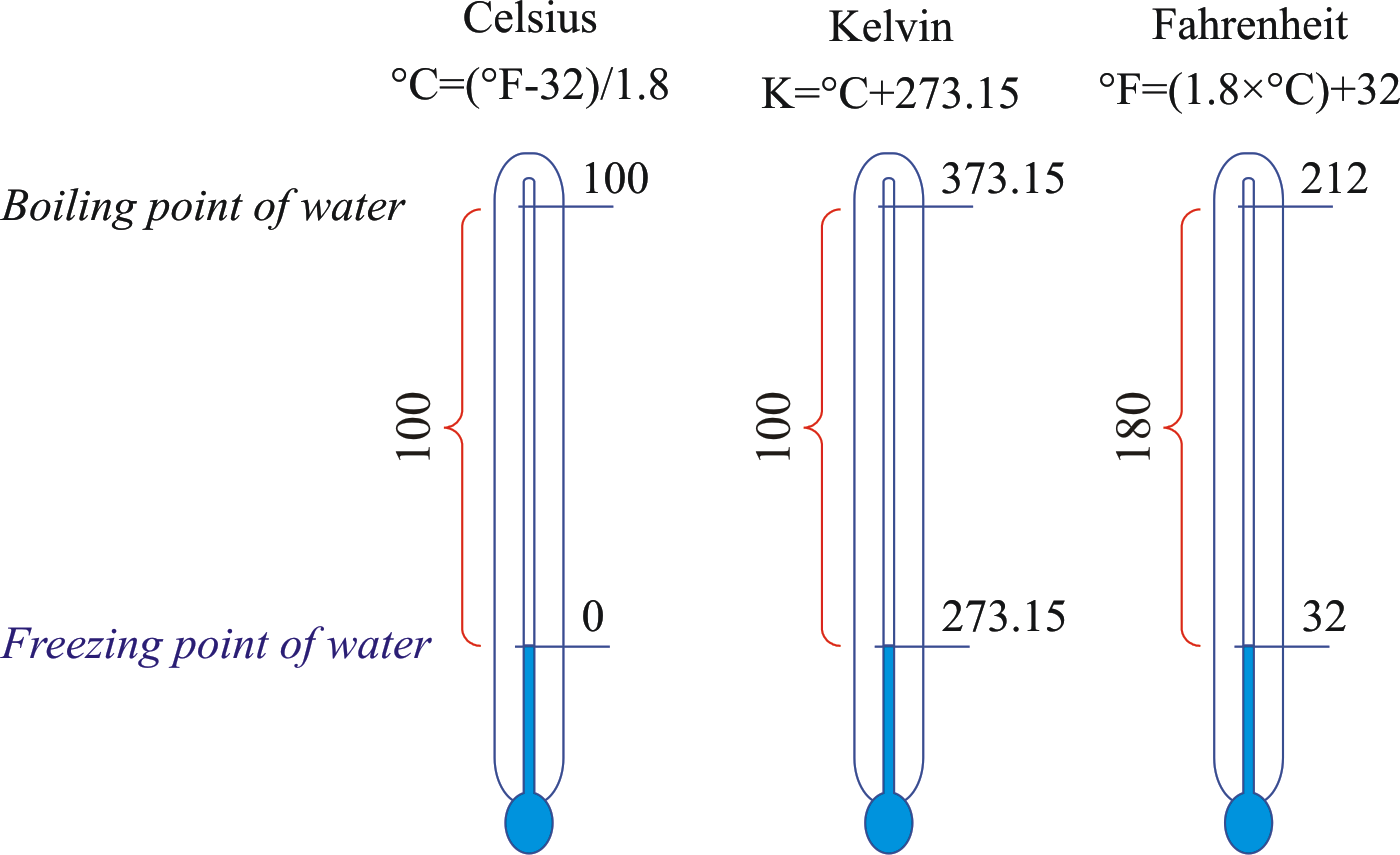
\includegraphics[width=7cm]{fig/temperature_scales.png}
            \newline
            \tiny{Tomado de \href{https://glossary.periodni.com/dictionary.php?en=logaritamska+skala}{aquí}}
        \end{column}
    \end{columns}
\end{frame}
\begin{frame}{Escalas de Temperatura}
\begin{table}[c]
    \centering
    \begin{tabular}{cccc}
        \toprule
        \textbf{Escala} & \textbf{Cero Absoluto} &\textbf{Fusión del hielo} & \textbf{Evaporación} \\
        \midrule
        \textbf{Kelvin} & $0\si{\kelvin}$ & $273\si{\kelvin}$ & $373.2\si{\kelvin}$ \\
        \textbf{Rankine} & $0\mathrm{R}$ & $491.7\mathrm{R}$ & $671.7\mathrm{R}$ \\
        \textbf{Reamur} & $-285.5\mathrm{Re}$ & $0\mathrm{Re}$ & $80\mathrm{Re}$ \\
        \textbf{Centígrada} & $-273.2\si{\celsius}$ & $0\si{\celsius}$ & $100\si{\celsius}$ \\
        \textbf{Farenheit} & $-459.7\si{\degree}\mathrm{F}$ & $32\si{\degree}\mathrm{F}$ & $212.0\si{\degree}\mathrm{F}$ \\
        \bottomrule
    \end{tabular}
    \caption{Distintas escalas de temperatura \cite{cengel2003termodinamica}} 
    \label{tab:limites}
\end{table}
\end{frame}
\begin{frame}{Conversión entre escalas}
\setlength{\extrarowheight}{4pt}
\begin{table}[c]
    \centering
    \begin{tabular}{|c|c|}
        \hline
        \textbf{Kelvin a Celsius} & \textbf{Kelvin a Farenheit}\\
        \Large{$\si{\celsius}=\si{\kelvin}-273.15$} & \Large{$\si{\degree}\mathrm{F}=\dfrac{9(\si{\kelvin}-273.15)}{5}+32$}\\[10pt]
        \hline
        \textbf{Farenheit a Celsius} & \textbf{Farenheit a Kelvin} \\
        \Large{$\si{\celsius}=\dfrac{5(\si{\degree}\mathrm{F}-32)}{9}$ } & \Large{$\si{\kelvin}=\dfrac{5(\si{\degree}\mathrm{F}-32)}{9}+273.15$}\\[10pt]
        \hline
        \textbf{Celsius a Kelvin} & \textbf{Celsius a Farenheit} \\
        \Large{$\si{\kelvin}=\si{\celsius}+273.15$ } & \Large{$\si{\degree}\mathrm{F}=\dfrac{9(\si{\celsius})}{5}+32$}\\[10pt]
        \hline
    \end{tabular}
    \caption{Distintas escalas de temperatura \cite{cengel2003termodinamica}}
    \label{tab:conversion}
\end{table}
\end{frame}
\begin{frame}{Formas de medición de temperatura}
\centering
\begin{tikzpicture}[mindmap,
  level 1 concept/.append style={level distance=80,sibling angle=90},
  extra concept/.append style={text=black}]
 
  % MATERIALES
  \path[mindmap,concept color=color_mate,text=black]
  node[concept] {\small{Medición Temperatura}}  [clockwise from=45]
  
    %
    % MATERIALES: PÉTREOS
    child[concept color= color_petr] {
      node[concept, inner sep = 0mm ] {Variación Volumen}  [clockwise from=0]
      child { node[concept, inner sep = 0mm ] {Termomé- tros} }
    }
    %
    % MATERIALES: TEXTILES
    child[concept color=color_text] {
      node[concept] {Intensidad Radiación} [clockwise from=0]
      child { node[concept] {Pirómetros} }
    }
    %
    % MATERIALES: METALES
    %
    % MATERIALES: PLÁSTICOS
    child[concept color=color_plas] { 
      node[concept] {Variación Resistencia} [clockwise from=180]
      child { node[concept] {RTD} }
    }
    %
    % MATERIALES: MADERA
    child[concept color=color_made] { 
      node[concept] {Generación f.e.m}  [clockwise from=180]
      child { node[concept] {Termopar} }
   };
 
\end{tikzpicture}
\end{frame}
\begin{frame}{Termómetros}
    \begin{columns}[c, onlytextwidth]
        \begin{column}{0.5\textwidth}
            \begin{itemize}
                \item El termómetro es uno de los instrumentos más utilizados para la medición de temperatura. 
                \item Se compone de dos partes importantes:
                \begin{itemize}
                    \item transductor de temperatura
                    \item escala numérica de conversión
                \end{itemize}
                \item Los principios sobre los que operan estos instrumentos son conocidos desde la cultura griega.
            \end{itemize}
        \end{column}
        \begin{column}{0.45\textwidth}
        \begin{figure}
            \centering
            \begin{tikzpicture}[
            node distance = 0.1cm and 0.1cm,
            every node/.style = {rectangle, font=\sffamily\bfseries, text=white,
                                 top color=blue!90!black, bottom color=blue!60!black,
                                 text width=2cm, align = center, minimum height = 1cm}
                                 ]
            \node (MAN)     {\small{Termómetro}};
            \node (PROD) [below left = of MAN] {\footnotesize{De vidrio}};
            \node (FIN)  [below right     = of MAN] {\footnotesize{Bimetálicos}};
            \node (CL)  [below right     = of PROD] {\footnotesize{Clínicos}};
            \node (IND)  [below    = of CL] {\footnotesize{Industriales}};
            %
            \draw [blue,thick]  (MAN) |- (FIN)
                                (MAN) |- (PROD)
                                (PROD) |- (CL)
                                (PROD) |- (IND);
    \end{tikzpicture}
            \caption{Tipos de termómetros \cite{sole2005instrumentacion}}
            \label{fig:term}
        \end{figure}
        
        \end{column}
    \end{columns}
\end{frame}
\begin{frame}{Termómetros de vidrio}
    \begin{columns}[c, onlytextwidth]
        \begin{column}{0.5\textwidth}
            \begin{itemize}
                \item Contiene un depósito de vidrio que contiene una sustancia, e.g. mercurio, y que al calentarse se expande y sube en el tubo capilar.  
                \item Márgenes de operación \cite{sole2005instrumentacion}
                \begin{itemize}
                    \item Mercurio: $-35\si{\celsius}$ hasta $280\si{\celsius}$
                    \item Mercurio (tubo capilar lleno de gas): $-35\si{\celsius}$ hasta $450\si{\celsius}$
                    \item Pentano: $-200\si{\celsius}$ hasta $20\si{\celsius}$
                    \item Alcohol: $-110\si{\celsius}$ hasta $50\si{\celsius}$
                    \item Tolueno: $-70\si{\celsius}$ hasta $100\si{\celsius}$
                \end{itemize}
            \end{itemize}
        \end{column}
        \begin{column}{0.45\textwidth}
            \centering
            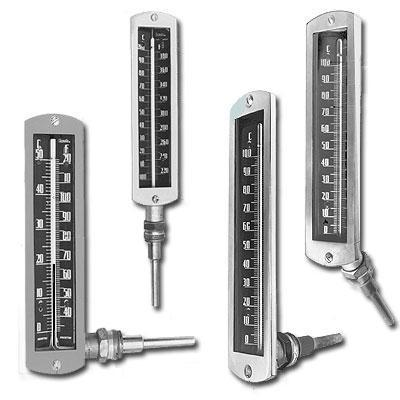
\includegraphics[width=6cm]{fig/TermometroVidrio.jpg}
             \\ \tiny{Tomado de \href{http://famater.com.ar/?p=611}{aquí}}
        \end{column}
    \end{columns}
\end{frame}
\begin{frame}{Termómetros bimetálicos}
    \begin{columns}[c, onlytextwidth]
        \begin{column}{0.5\textwidth}
            \begin{itemize}
                \item Se basan en el distinto coeficiente de dilatación de dos metales diferentes \textit{e.g.}latón y una aleacción de ferroníquel. 
                \item La diferencia en el coeficiente de expasión de cada metal hace que el elemento bimetálico se doble. 
                \item La exactitud del instrumento es de $1\%$ y su campo de medida es de $-200\si{\celsius}$ hasta $500\si{\celsius}$
            \end{itemize}
        \end{column}
        \begin{column}{0.45\textwidth}
            \centering
            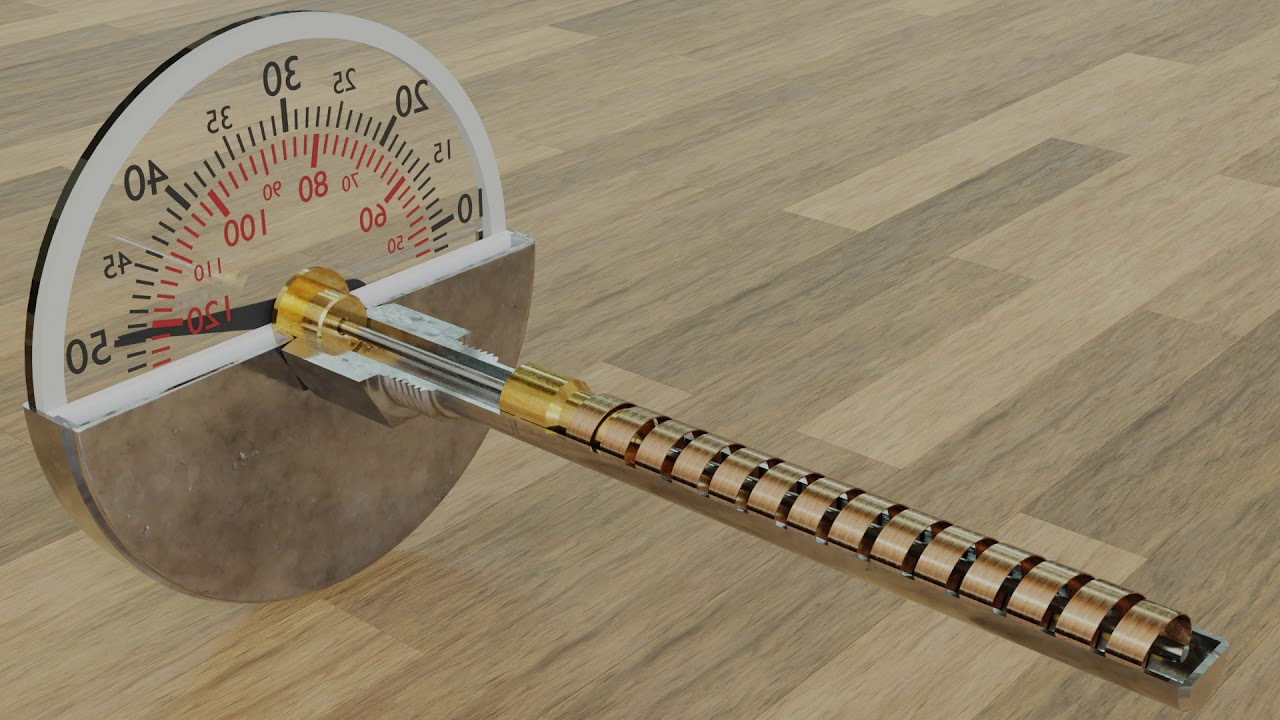
\includegraphics[width=5cm]{fig/bimetalic.png}
             \\ \tiny{Tomado de \href{https://natstuk.com/?p=786}{aquí}}
        \begin{equation*}
                \alpha = \dfrac{360}{\pi}\cdot \dfrac{a \cdot l}{s}\cdot (t_2-t_1) 
        \end{equation*}
        \end{column}
    \end{columns}
\end{frame}
\begin{frame}{Termopares(Termocuplas)}
    \begin{columns}[c, onlytextwidth]
        \begin{column}{0.55\textwidth}
            \begin{itemize}
                \item Se basa en el efecto Seebeck (Thomas Seebeck, 1821). 
                \item Un termopar, se componen dos metales diferentes cuyas uniones, producen una pequeña tensión cuando la junta se calienta. 
                \item Está tensión solo depende de las características de los materiales y la temperatura. 
            \end{itemize}
        \end{column}
        \begin{column}{0.40\textwidth}
        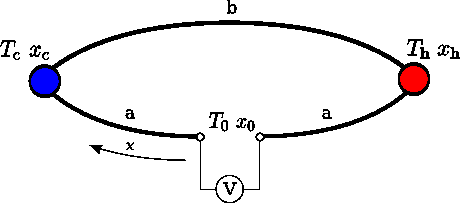
\includegraphics[width=6cm]{fig/seebeekc.png}
            \tiny{Tomado de \href{https://www.iue.tuwien.ac.at/phd/mwagner/node14.html}{aquí}}
        \end{column}
    \end{columns}
\end{frame}
\begin{frame}{Leyes de los termopares}
    Se caracterizan por tres leyes fundamentales:\\[8pt]
    \begin{itemize}
        \item \emph{Ley de circuito homogéneo: } En un conductor metálico homogéneo no puede sostenerse la circulación de una corriente eléctrica por la aplicación exclusiva de calor.
        \item \emph{Ley de las temperaturas intermedias: } En un termopar con las juntas de los metales A y B a las temperaturas T1 y T2 la fem termoeléctrica generada es independiente de las temperaturas intermedias en los conductores A y B.
        \begin{center}
            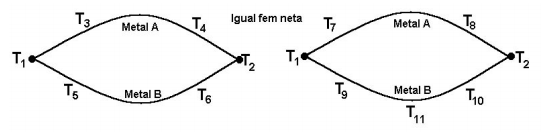
\includegraphics[width=10cm]{fig/ley2.PNG}
        \end{center}
    \end{itemize}
    \tiny{Tomado de \href{http://laboratorios.fi.uba.ar/lscm/termocuplas01.pdf}{aquí}}
\end{frame}
\begin{frame}{Leyes de los termopares}
    Continua...\\[8pt]
    \begin{itemize}
        \item \emph{Ley de los metales intermedios: } Si en un termopar insertamos un segmento de conductor de un tercer metal C , en alguno de los dos conductores metálicos A ó B, la fem generada será independiente de la existencia de este tercer conductor siempre que las temperaturas de las juntas del mismo sean iguales. 
        \begin{center}
            \includegraphics[width=10cm]{fig/ley3.PNG}
        \end{center}
    \end{itemize}
    \tiny{Tomado de \href{http://laboratorios.fi.uba.ar/lscm/termocuplas01.pdf}{aquí}}
\end{frame}
\begin{frame}{Termopares(Termocuplas)}
    \begin{columns}[c, onlytextwidth]
        \begin{column}{0.45\textwidth}
            \begin{itemize}
                \item El diamétro de los cables varia entre 0.1 y 3mm. A menor diámetro mayor tiempo de respuesta. 
                \item La selección de los alambres para termopares se hace de forma que tengan una resistencia eléctrica y que el aumento de \textit{f.e.m} sea paralelo al aumento de temperatura.
                \item Existen distintos tipos de acople de temperatura.
                
            \end{itemize}
        \end{column}
        \begin{column}{0.5\textwidth}
            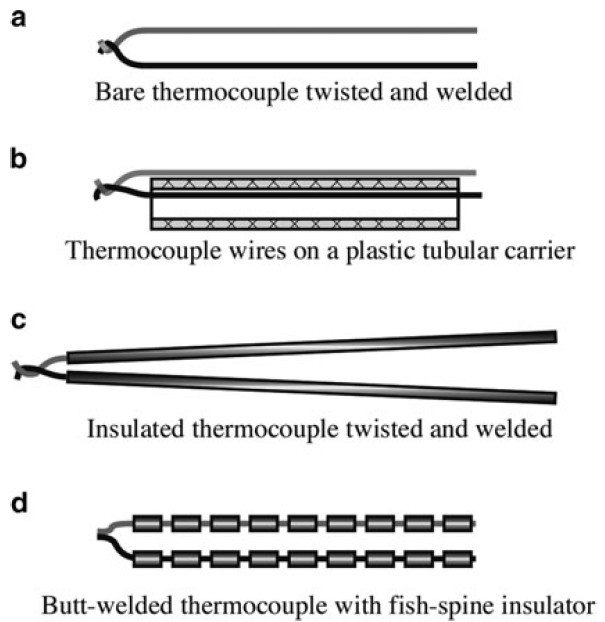
\includegraphics[width=6cm]{fig/ensamble_termopar.PNG}
            \\ \cite{Fraden_2016}
        \end{column}
    \end{columns}
\end{frame}
\begin{frame}{Tipos de termopares}
\centering
    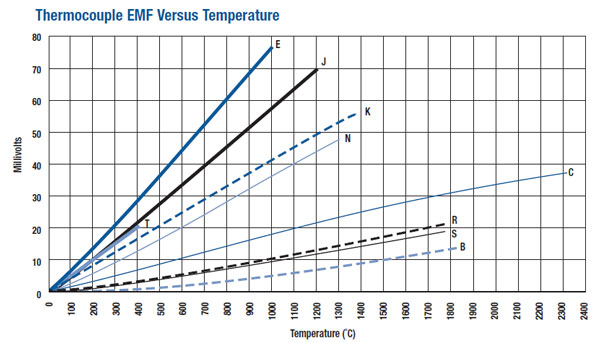
\includegraphics[width=11.5cm]{fig/Thermocouple_EMF_Temperature.png}
     \\ \tiny{Tomado de \href{https://www.akcp.com/blog/what-is-a-k-type-thermocouple/}{aquí}}
\end{frame}
\begin{frame}{Tipos de termopares}
  \begin{table}[]
    \centering
    \footnotesize{
    \begin{tabular}{m{0.6cm} m{3.4cm} c c m{3.8cm}}
        \toprule
        \textbf{Tipo} & \textbf{Material} &\textbf{Rango medida} & \textbf{Rango trabajo} & \textbf{Uso} \\
        &  &  \centering[\si{\celsius}] & \centering[\si{\celsius}] & \\
        \midrule
        \textbf{E} & Cromel-Constatán & $-100\sim 1270$ & $-40\sim 900$ & Puede usarse en vacío\\
        \textbf{T} & Cobre-Constatán & $-200\sim  371$ & $-40\sim 350$ & Resiste la corrosión\\
        \textbf{J} & Hierro-Constatán & $-190\sim  760$ & $-40\sim 750$ & Atmósferas inertes.\\
        \textbf{K} & Cobre-Alumel & $-190\sim  1260$ & $-40\sim 1000$ & Atmósferas oxidantes\\
        \textbf{R} & Platino-Rodio & $0\sim  1450$ & $0\sim 1200$ & Atmósferas oxidantes\\
        \textbf{S} & Platino-Rodio & $0\sim  1450$ & $0\sim 1200$ & Similar a R\\
        \textbf{B} & Platino-Rodio & $0\sim  1950$ & $0\sim 1800$ & Altas Temperaturas\\
        \textbf{N} & Cobre-Constatán & $0\sim  2316$ & $0\sim 2100$ & Sustituto de K\\
        \bottomrule
    \end{tabular}
    }
    \caption{Comparación entre distintos tipos de sensores\cite{sole2005instrumentacion}}
    \label{tab:Comparacion_termo}
\end{table}
\end{frame}
\begin{frame}{Tipos de termopares \tiny{\href{https://srdata.nist.gov/its90/download/download.html}{https://srdata.nist.gov/its90/download/download.html}}}
\centering
    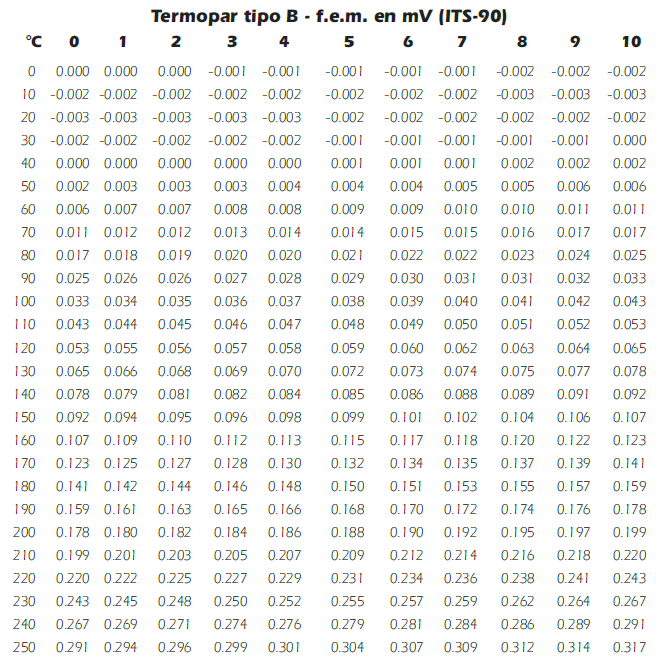
\includegraphics[width=11cm]{fig/ITS-90.PNG}
\end{frame}
\begin{frame}{Tipos de termopares}
\centering
    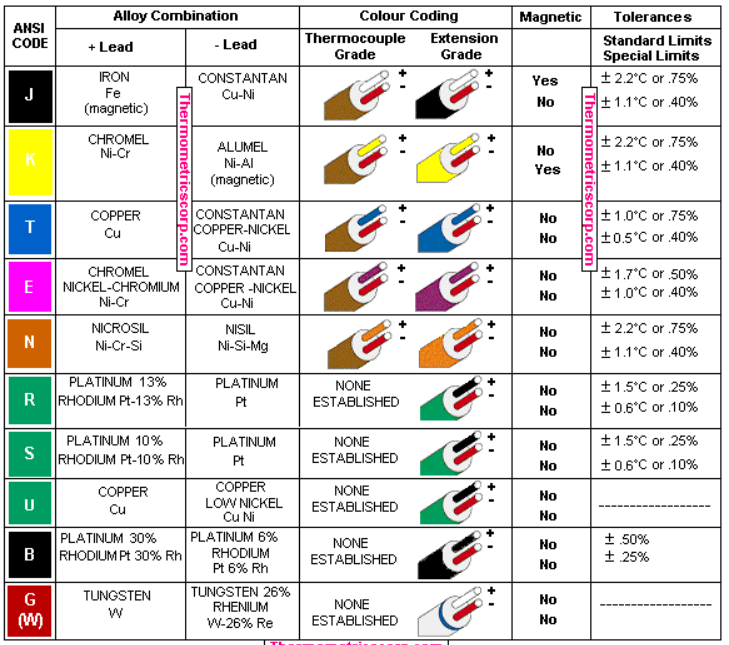
\includegraphics[width=7.5cm]{fig/thermometricscorp.png}
    \\ \tiny{Tomado de \href{https://www.thermometricscorp.com/thermocouple-color-code.html}{aquí}}
\end{frame}
\begin{frame}{Tubos de protección}
\centering
    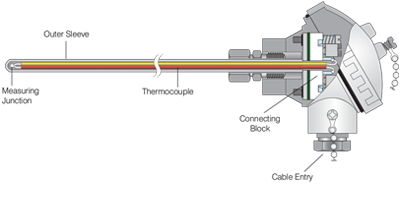
\includegraphics[width=11cm]{fig/thermocouple-probe-head.png}
    \\ \tiny{Tomado de \href{https://www.tcaus.com.au/thermocouple/index.html}{aquí}}
\end{frame}
\begin{frame}{Lectura de datos termocoupla}
 \begin{columns}[c, onlytextwidth]
        \begin{column}{0.45\textwidth}
            \begin{itemize}
                \item El voltaje de salida es muy bajo, por lo que se requiere un sistema de acondicionamiento de la señal, para amplificar dicha señal.  
                \item La sensibilidad es muy baja. Pero presentan una respuesta muy lineal. Además no requieren alimentación de ningún tipo.
                \item El sistema a de acondicionamiento selecciona en función del sensor. 
                
            \end{itemize}
        \end{column}
        \begin{column}{0.5\textwidth}
            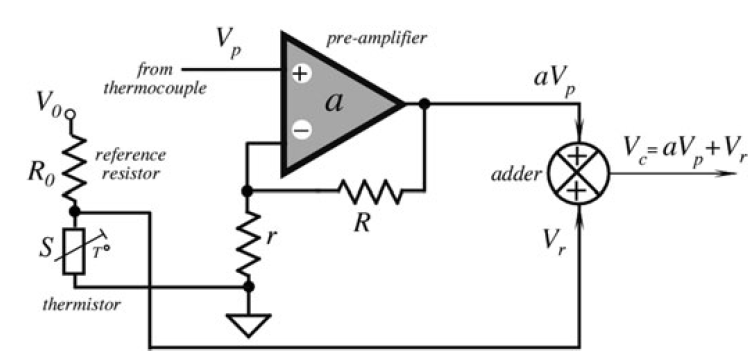
\includegraphics[width=7cm]{fig/thermocouple_circuit.PNG}
            \\ \cite{Fraden_2016}
        \end{column}
    \end{columns}
\end{frame}
\begin{frame}{Compensación de la unión fría (CJC)}
 \begin{columns}[c, onlytextwidth]
        \begin{column}{0.45\textwidth}
            \begin{itemize}
                \item Los voltajes de referencia están referidas a una unión fría, por lo que se requiere una compensación.  
                \item Esta compensación se puede realizar de varias maneras, incluso en software. 
                \item Siempre es necesario integrar este tipo de integración de sistemas de adquisición de datos (recientemente se puede realizar de forma digital)
            \end{itemize}
        \end{column}
        \begin{column}{0.5\textwidth}
            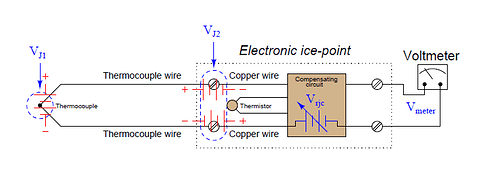
\includegraphics[width=8.5cm]{fig/Thermocouple_cjc.png}
            \\ \tiny{Tomado de \href{https://forumautomation.com/t/what-is-cold-junction-compensation-in-thermocouple/2896}{aquí}}
        \end{column}
    \end{columns}
\end{frame}
\begin{frame}{Detector de temperatura por Resistencia (RTD)}
    \begin{columns}[c, onlytextwidth]
        \begin{column}{0.55\textwidth}
            \begin{itemize}
                \item Estos detectores de temperatura dependen de la variación de la resistencia del material en función de la temperatura.  
                \item El elemento consiste en un arrollamiento de hilo muy fino del conductor adecuado bobinado entre capas de material aislante y protegido con un revestimiento de vidrio o cerámica. 
                \item Relación dada por: 
                \begin{equation*}
                    R_T=R_0\cdot (1+\alpha \cdot T)
                \end{equation*}
            \end{itemize}
        \end{column}
        \begin{column}{0.45\textwidth}
            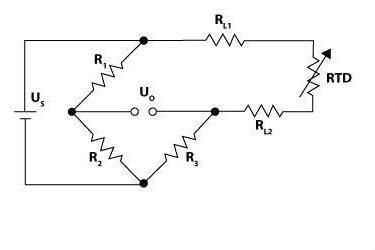
\includegraphics[width=6cm]{fig/RTD_Circuit.jpg}
            \\ \tiny{Tomado de \href{https://www.azom.com/article.aspx?ArticleID=5573}{aquí}}
        \end{column}
    \end{columns}
\end{frame}
\begin{frame}{Fabricación RTD}
    \begin{columns}[c, onlytextwidth]
        \begin{column}{0.45\textwidth}
        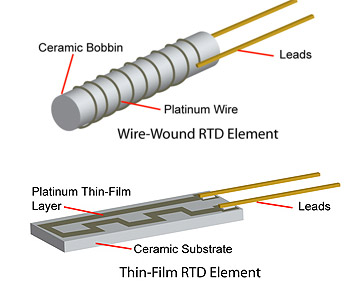
\includegraphics[width=6.5cm]{fig/rtd_types.jpg}
            \\ \tiny{Tomado de \href{https://www.designworldonline.com/designing-with-rtd-temperature-sensors/}{aquí}}
            
        \end{column}
        \begin{column}{0.55\textwidth}
            \begin{itemize}
                \item \textbf{Hilo bobinado}: el embobinado de platino es soportado por un vidrio resistente de alta temperatura dentro de un tubo de cerámica.     
                \item \textbf{Película fina}:Regularmente fabricados de platino y aceros que son depositados en una membrana de silicio.
            \end{itemize}
        \end{column}
    \end{columns}
\end{frame}
\begin{frame}{Características sondas RTD}
  \begin{table}[]
    \centering
    \scriptsize{
    \begin{tabular}{m{1.1cm} m{2.2cm} m{1.5cm} m{1.8cm} m{2.6cm} m{2.6cm}}
    \toprule
        \textbf{Elemento} & \textbf{Intervalo Útil} &\textbf{Resistencia básica} & \textbf{Sensibilidad [$\Omega/\si{\celsius}$ de $0\si{\celsius}$ a $100\si{\celsius}$]} & \textbf{Ventajas} & \textbf{Desventajas}\\
    \midrule
       \textbf{Platino} & $-260\si{\celsius}$ a $ 850\si{\celsius}$ & $100\Omega$ a $0\si{\celsius}$   & 0,39 & Mayor intervalo, mejor estabilidad, buena linealidad & Costo\\
       \textbf{Cobre} & $-100\si{\celsius}$ a $ 260\si{\celsius}$ & $10\Omega$ a $25\si{\celsius}$   & 0,04 & Buena linealidad & Baja resistividad\\
       \textbf{Níquel} &  $-100\si{\celsius}$ a $ 260\si{\celsius}$ & $100\Omega$ a $0\si{\celsius}$   & 0,62 & Bajo Costo, Alta sensibilidad & Falta de linealidad, variaciones coeficiente de resistencia\\
       \textbf{Níquel-Hierro} & $-100\si{\celsius}$ a $ 204\si{\celsius}$ & $604\Omega$ a $0\si{\celsius}$   & 3,13 & Bajo costo, muy alta sensibilidad & Relación reducida\\
    \bottomrule
    \end{tabular}
    }
    \caption{Comparación entre distintos tipos de sensores\cite{sole2005instrumentacion}}
    \label{tab:Caracteristicas _rtd}
\end{table}
\end{frame}
\begin{frame}{Estándar de tolerancias RTD}
 \begin{itemize}
     \item Los RTD son construidos bajo distintos estándares y curvas. La más común es la DIN/IEC 60751.
     \item Este estándar divide por clases en función de la respuesta de la resistencia del platino por temperatura. 
     \item \textbf{Clase A}
     \begin{itemize}
         \item Tolerancia de Temperatura: $\pm (0.15 + .002|T| \si{\celsius} C)$
     \end{itemize}
      \item \textbf{Clase B}
     \begin{itemize}
         \item Tolerancia de Temperatura: $\pm (0.30 + .005|T| \si{\celsius} C)$
         \end{itemize}
    \item \textbf{Clase C}
     \begin{itemize}
         \item Tolerancia de Temperatura: $\pm (1.2 + .005|T| \si{\celsius} C)$
     \end{itemize}
 \end{itemize}
\end{frame}
\begin{frame}{Algunas consideraciones RTD}
    \begin{columns}[c, onlytextwidth]
    \begin{column}{0.55\textwidth}
            \begin{itemize}
                \item Son especiales en precisión en linealidad.      
                \item No se requieren recalibraciones anuales, y se mantienen estables por muchos años. 
                \item Requieren una fuente de corriente precisa. 
            \end{itemize}
        \end{column}
        \begin{column}{0.45\textwidth}
        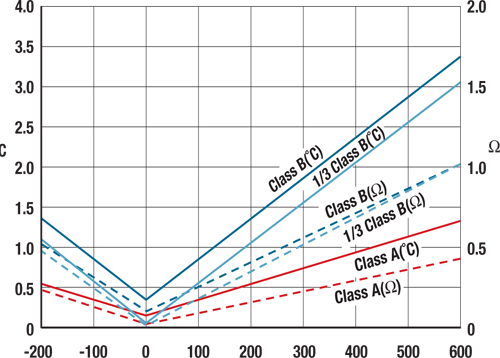
\includegraphics[width=6.5cm]{fig/RTD Curve.jpg}
            \\ \tiny{Tomado de \href{http://www.bearingsensor.com/bearing-rtd.html}{aquí}}
            
        \end{column}
        
    \end{columns}
\end{frame}
\begin{frame}{Conexiones RTD (2 hilos)}
    \begin{columns}[c, onlytextwidth]
    \begin{column}{0.50\textwidth}
        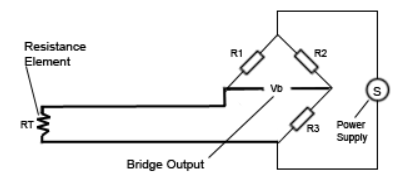
\includegraphics[width=7cm]{fig/2hilosRTD.PNG}
            \\ \tiny{Tomado de \href{http://www.bearingsensor.com/bearing-rtd.html}{aquí}}
            
        \end{column}
    \begin{column}{0.55\textwidth}
            \begin{itemize}
                \item Proporciona una conexión eléctrica a la salida de cada elemento.     
                \item Solución más económica
                \item Requieren una fuente de corriente precisa. 
            \end{itemize}
        \end{column}
    \end{columns}
\end{frame}
\begin{frame}{Conexiones RTD (3 hilos)}
    \begin{columns}[c, onlytextwidth]
    \begin{column}{0.55\textwidth}
            \begin{itemize}
                \item Se obtiene mayor precisión, ya que se contrarrestra el efecto del puente de \textit{Wheatstone}     
                \item Es la forma más utilizada en la industria.
                \item El cable 3 no conduce corriente.
            \end{itemize}
        \end{column}
        \begin{column}{0.45\textwidth}
        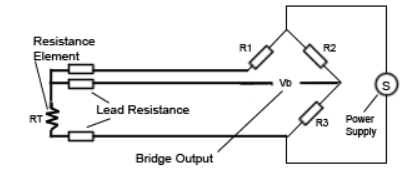
\includegraphics[width=7cm]{fig/3hilosRTD.PNG}
            \\ \tiny{Tomado de \href{http://www.bearingsensor.com/bearing-rtd.html}{aquí}}
            
        \end{column}
        
    \end{columns}
\end{frame}
\begin{frame}{Conexiones RTD (4 hilos)}
    \begin{columns}[c, onlytextwidth]
        \begin{column}{0.45\textwidth}
        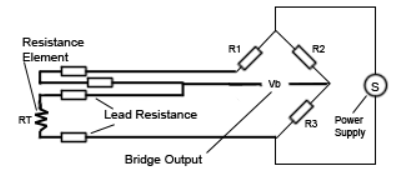
\includegraphics[width=6.5cm]{fig/4hilosRTD.PNG}
            \\ \tiny{Tomado de \href{http://www.bearingsensor.com/bearing-rtd.html}{aquí}}
            
        \end{column}
    \begin{column}{0.55\textwidth}
            \begin{itemize}
                \item Son especiales en precisión en linealidad.      
                \item No se requieren recalibraciones anuales, y se mantienen estables por muchos años. 
                \item Requieren una fuente de corriente precisa. 
            \end{itemize}
        \end{column}
        
    \end{columns}
\end{frame}
\begin{frame}{Termistores}
    \begin{columns}[c, onlytextwidth]
        \begin{column}{0.55\textwidth}
            \begin{itemize}
                \item Es una contracción de las palabras \textit{thermal} y \textbf{resistor} 
                \item Este tipo de medidores son semiconductores de partículas de óxido de metal. 
                \item Existen dos grupos: \textit{NTC (Negative Temperature Coeficient) } y \textit{PTC (Positive Temperature Coeficient)}
            \end{itemize}
        \end{column}
        \begin{column}{0.40\textwidth}
           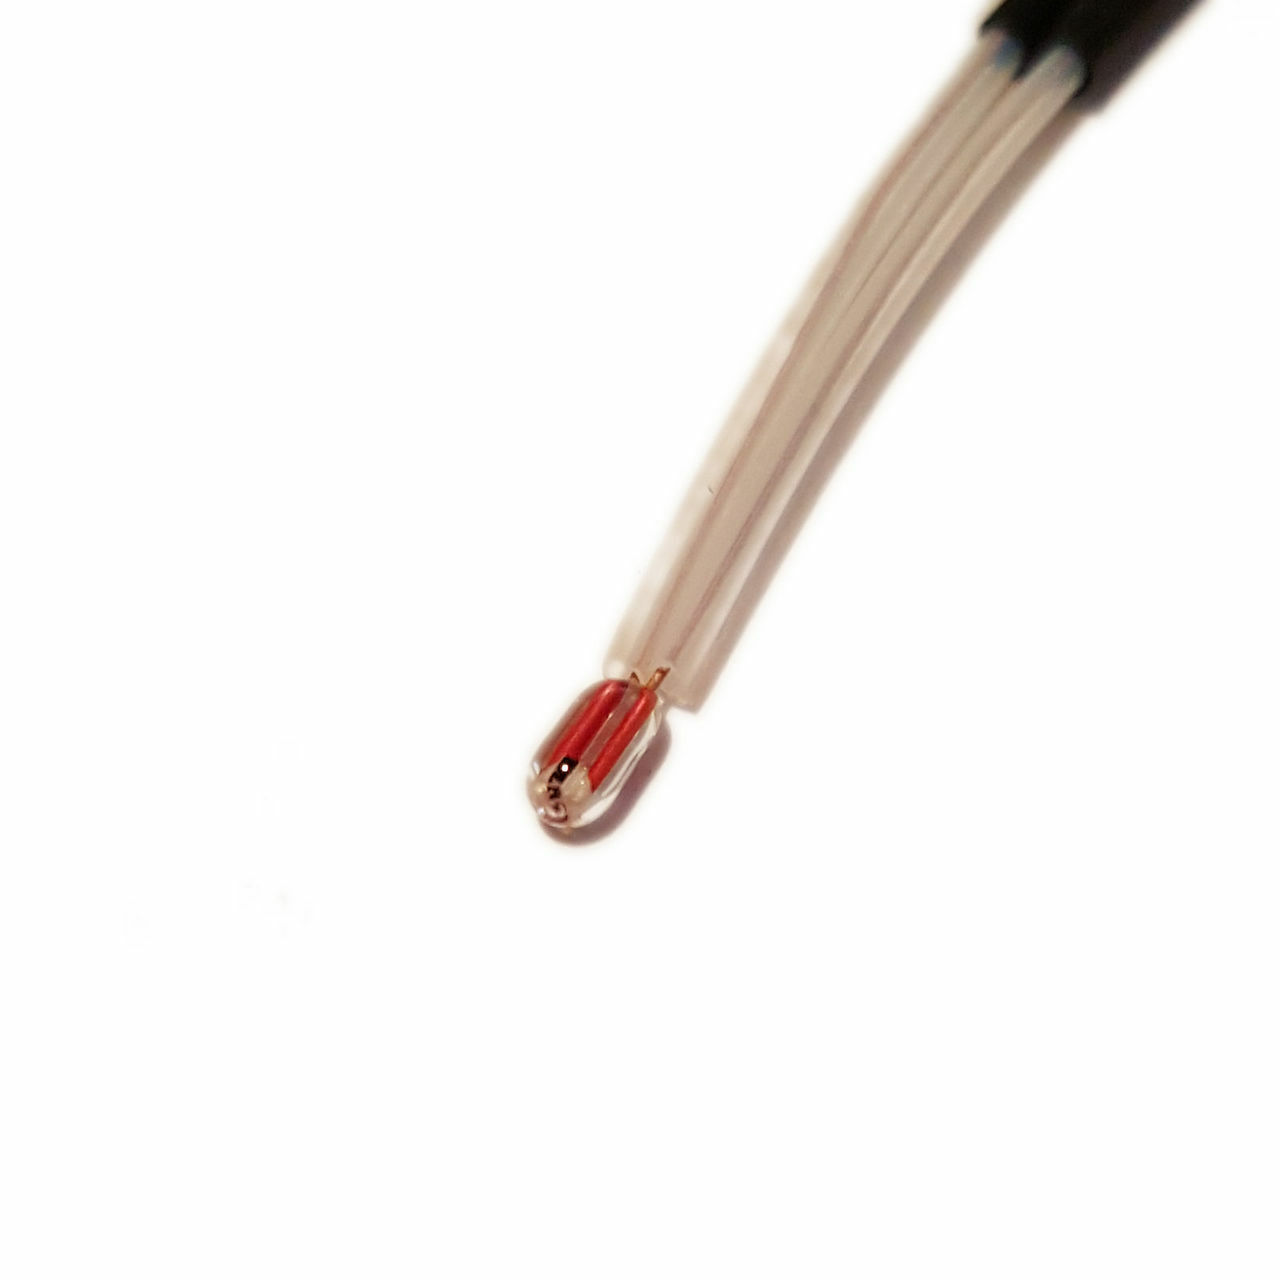
\includegraphics[width=6.5cm]{fig/thermistor_NTC_100K.jpg}
            \\ \tiny{Tomado de \href{https://spool3d.ca/ntc-100k-thermistor-with-terminal/}{aquí}}
        \end{column}
    \end{columns}
\end{frame}
\begin{frame}{Curvas Termistores}
    \begin{columns}[c, onlytextwidth]
        \begin{column}{0.55\textwidth}
             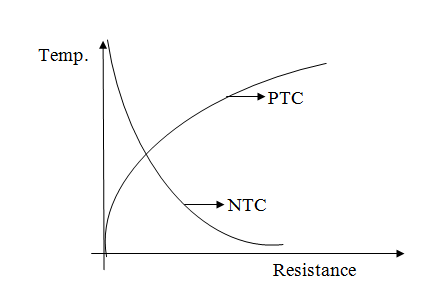
\includegraphics[width=8cm]{fig/Thermistor_Curve.png}
            \\ \tiny{Tomado de \href{https://www.researchgate.net/publication/309267235_A_Simple_Thermistor_Design_for_Industrial_Temperature_Measurement/figures?lo=1&utm_source=google&utm_medium=organichttps://spool3d.ca/ntc-100k-thermistor-with-terminal/}{aquí}}
        \end{column}
        \begin{column}{0.40\textwidth}
        \begin{equation*}
            R_t=R_0e^{\beta(\frac{1}{T_1})(\frac{1}{T_2})}
        \end{equation*}
        
        \begin{equation*}
            \frac{1}{T}=A+B\cdot \ln R_1 + C \cdot (\ln R_1)^3
        \end{equation*}
          
        \end{column}
    \end{columns}
\end{frame}
\begin{frame}{Termistores}
    \begin{columns}[c, onlytextwidth]
        \begin{column}{0.55\textwidth}
            \begin{itemize}
                \item Se les denominad \textit{Sensor on a chip} por su tamaño reducido y facilidad para encapsular en vidrio o epoxi.
                \item Su tiempo de respuesta depende de la capacidad térmica y masa del termistor, variando de 0,5 a 10 segundos.  
                \item La precisión de un termistor se encuentra entre $\pm 0.1 {\si{\celsius}}$ a $\pm 0.2 {\si{\celsius}}$. Con un rango de $-50 {\si{\celsius}}$ a $200 {\si{\celsius}}$.
                \item Se usan para la protección contra calentamiento de PC, baterías de litio o regular contraste en un LCD. 
            \end{itemize}
        \end{column}
        \begin{column}{0.40\textwidth}
           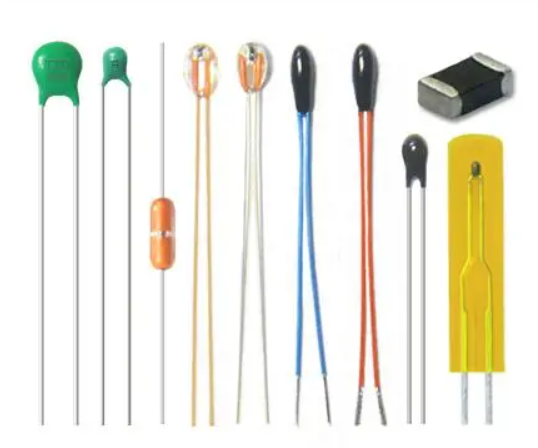
\includegraphics[width=6.5cm]{fig/Thermistor_type.PNG}
            \\ \tiny{Tomado de \href{https://es.made-in-china.com/co_jpsensor/product_Ntc-10K-Thermistor-Collection_reeeohegg.html}{aquí}}
        \end{column}
    \end{columns}
\end{frame}
\begin{frame}{Medición de termistores}
    \begin{columns}[c, onlytextwidth]
            \begin{column}{0.5\textwidth}
           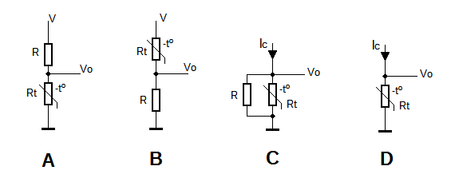
\includegraphics[width=7.5cm]{fig/450px-LinealizacionNTC.png}
            \\ \tiny{Tomado de \href{https://es.made-in-china.com/co_jpsensor/product_Ntc-10K-Thermistor-Collection_reeeohegg.html}{aquí}}
        \end{column}
        
        \begin{column}{0.45\textwidth}
            \begin{itemize}
                \item La curva de un termistor no es lineal. 
                \item Con circuitos sencillos se puede linealizar su característica de forma deseable.
                \item Se requiere de una fuente de precisión y una resistencia fija de precisión también.
                \item La fuente puede ser de corriente también.
            \end{itemize}
        \end{column}

    \end{columns}
\end{frame}
\begin{frame}{Pirómetros}
    \begin{columns}[c, onlytextwidth]
        \begin{column}{0.55\textwidth}
            \begin{itemize}
                \item Este tipo de dispositivos se utiliza por medios eléctricos y sin contacto.
                \item Se clasifican en función del fenómeno físico: 
                \begin{itemize}
                    \item Pirómetros de radiación
                    \item Pirómetro ópticos
                    \item De resistencia y termoeléctricos
                \end{itemize}
            \end{itemize}
        \end{column}
        \begin{column}{0.40\textwidth}
            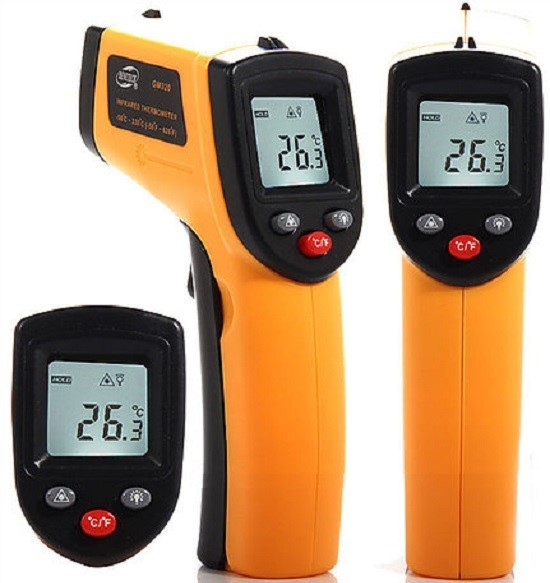
\includegraphics[width=5.5cm]{fig/Pirometro.jpg}
            \\ \tiny{Tomado de \href{https://como-funciona.co/un-pirometro/}{aquí}}
        \end{column}
    \end{columns}
\end{frame}
\begin{frame}{Pirómetros de radiación}
    \begin{columns}[c, onlytextwidth]
        \begin{column}{0.55\textwidth}
            \begin{itemize}
                \item Se fundan en la ley de Stefan-Boltzmann, que dice que la intensidad de energía radiante emitida por la superficie de un cuerpo aumenta proporcionalmente a la cuarta potencia de la temperatura absoluta (Kelvin) del cuerpo.
                \begin{equation*}
                    W= K \times T^4
                \end{equation*}
                \item El pirómetro dirigido sobre una superficie incandescente no nos dará su verdadera temperatura si la superficie no es perfectamente negra, es decir, que absorba absolutamente todas las radiaciones y no refleje ninguna.
            \end{itemize}
        \end{column}
        \begin{column}{0.45\textwidth}
            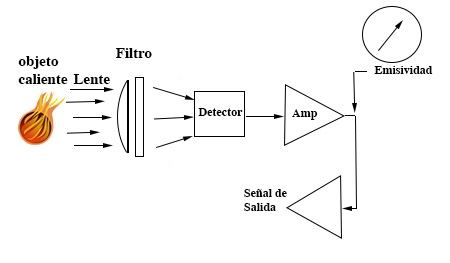
\includegraphics[width=7cm]{fig/pirometro-basico.jpg}
            \\ \tiny{Tomado de \href{https://www.ingmecafenix.com/otros/pirometro/}{aquí}}
        \end{column}
    \end{columns}
\end{frame}
\begin{frame}{Pirómetros ópticos}
    \begin{columns}[c, onlytextwidth]
        \begin{column}{0.47\textwidth}
            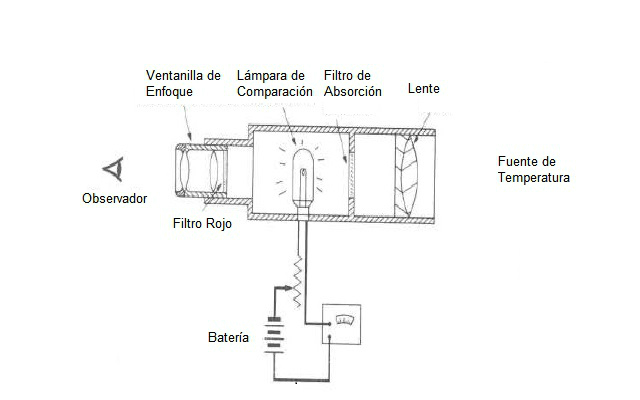
\includegraphics[width=8.5cm]{fig/Pirometros-optico-esquema.jpg}
            \\ \tiny{Tomado de \href{https://como-funciona.co/un-pirometro/}{aquí}}
        \end{column}
        \begin{column}{0.50\textwidth}
            \begin{itemize}
                \item Se basan en la comparación visual de la luminosidad del objeto radiante con el filamento de una lámpara incandescente.
                \item El sistema óptico del pirómetro restringe el ancho de onda de $\SI{0.65}{\micro\meter}$ a $\SI{0.66}{\micro\meter}$ (zona roja del espectro) y dispone de filtros para reducir la intensidad de la radiación recibida, permitiendo la medida de un amplio margen de temperaturas. 
                \item La exactitud de los pirómetros ópticos es del $\pm 1\%$ al $\pm2\%$ 
            \end{itemize}
        \end{column}
        
    \end{columns}
\end{frame}
\begin{frame}{Criterios de Selección}
 \begin{columns}[c, onlytextwidth]
        \begin{column}{0.40\textwidth}
        \centering
            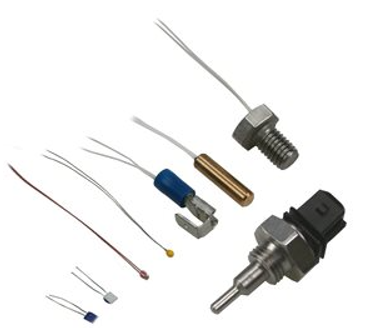
\includegraphics[width=7cm]{fig/Criteria Sensor.PNG}
            \\ \tiny{Tomado de \href{https://www.variohm.com/news-media/technical-blog-archive/selecting-temperature-sensor-things-to-consider}{aquí}}
        \end{column}
        \begin{column}{0.50\textwidth}
               \centering
    \diagram{Criterios selección}
        {- Exactitud \\
        - Rango \\
        - Estabilidad \\
        - Instalación\\
        - Costo\\
        - Ambiente
        }
        \end{column}
    \end{columns}
\end{frame}
\begin{frame}{Criterios de Selección}
    \centering
    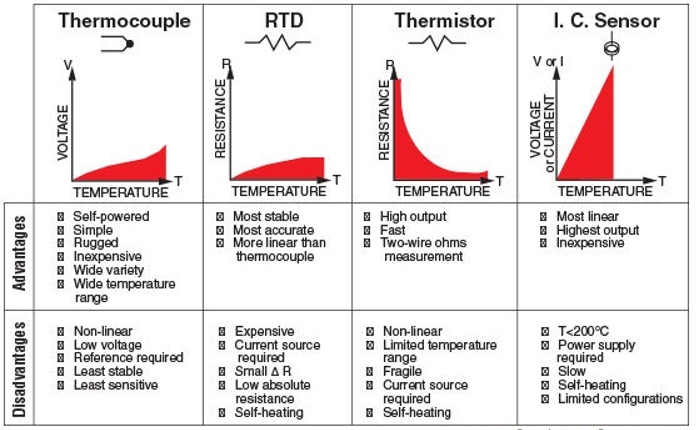
\includegraphics[width=11cm]{fig/Selection_Sensor.PNG}
            \\ \tiny{Tomado de \href{https://www.mechaterrain.com/lm35-temperature-sensor}{aquí}}
\end{frame}
\begin{frame}{Criterios de Selección}
  \begin{table}[]
    \centering
    \begin{tabular}{m{2cm} m{1.5cm} m{1.55cm} m{2cm} m{1.4cm}}
        \toprule
        \textbf{Tipo de Sensor} & \textbf{Exactitud} &\textbf{Rango típico} & \textbf{Tiempo de respuesta} & \textbf{Costo} \\
        \midrule
        \textbf{Termopares} & Baja & -200$\si{\celsius}$ a 1800$\si{\celsius}$ & 1 $s$ & Bajo\\
        \textbf{RTD Clase A, Estándar IEC} & Alta & -200$\si{\celsius}$ a 800$\si{\celsius}$ & 1-5 $s$ & Alto\\
        \textbf{Termistor NTC} & Alta & -200$\si{\celsius}$ a 1800$\si{\celsius}$ & < 1 $s$ & Alto\\
        \textbf{Sensores Infrarrojos} & Mediana & -20$\si{\celsius}$ a 1370$\si{\celsius}$ & < 1 $s$ & Bajo \\
        \bottomrule
    \end{tabular}
    \caption{Comparación entre distintos tipos de sensores}
    \label{tab:Comparacion}
\end{table}
\end{frame}
\begin{frame}{Referencias}
\bibliographystyle{ieeetr}
\footnotesize
\bibliography{comunes/referencias}
\end{frame}

\end{document}